\section{Non-rigid registration}
We can now perform a non-rigid transformation of two lung pairs in python. In \autoref{registration} we see the two images used along the results of the registration using MI and NCC. The male lungs have been chosen as the moving image for both registrations and the female lungs as the fixed image. This means the male lungs are transformed to match the female lungs. 

\begin{figure}[h]
	\centering
	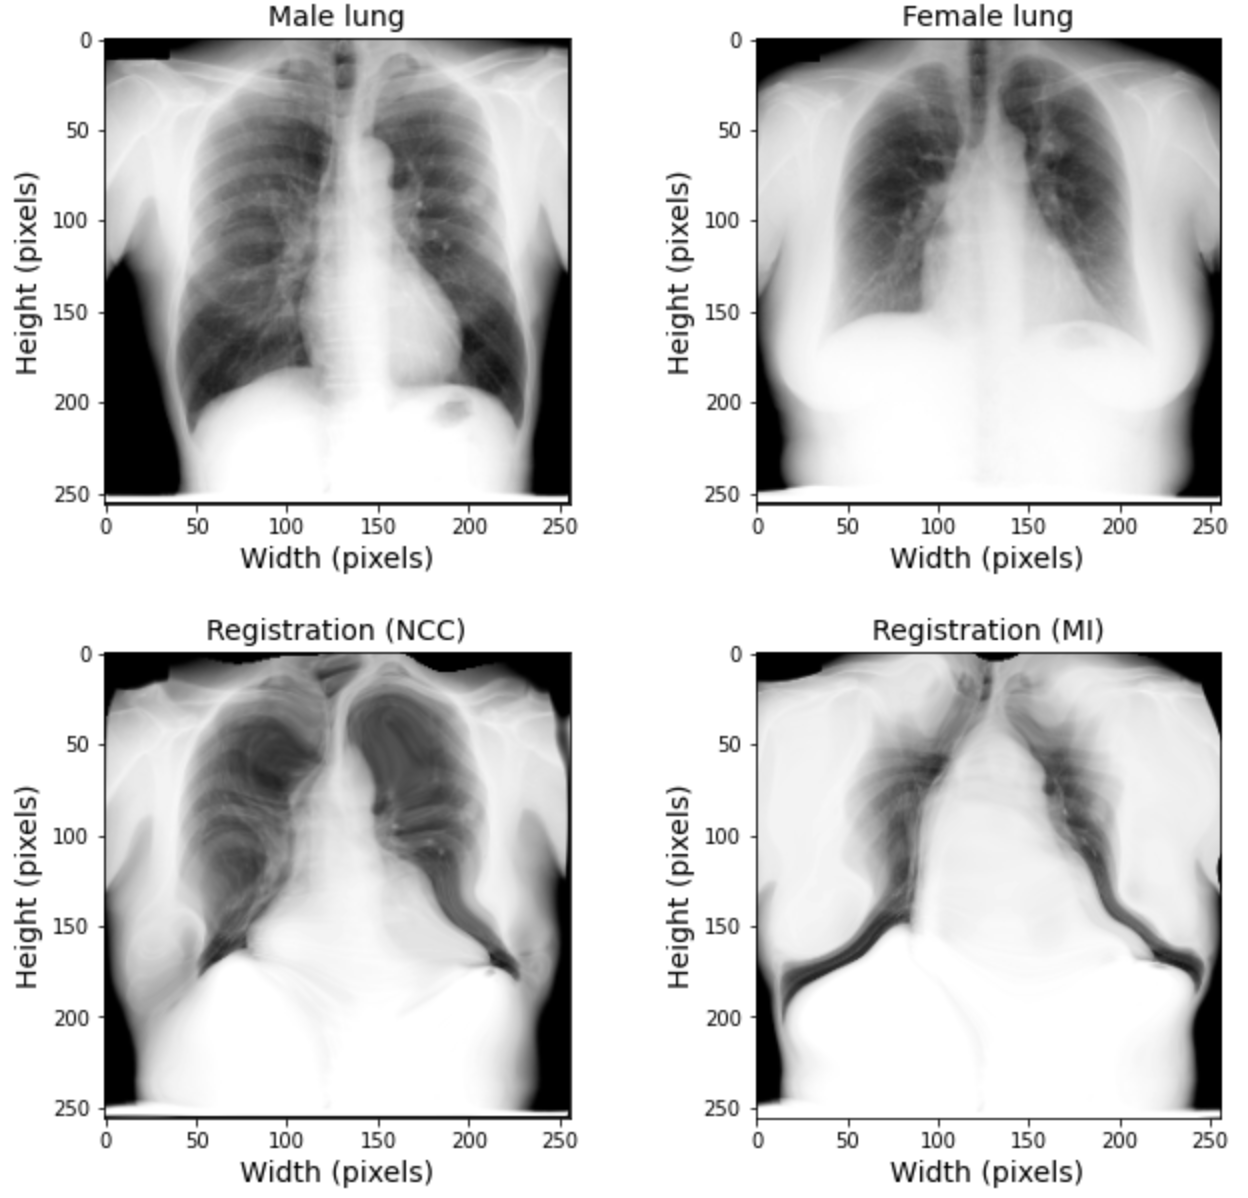
\includegraphics[width=0.8\linewidth]{Materials/registration}
	\caption{Top left: male lungs which will get registered to the female lungs. Top right: female lungs. Bottom left: result of registration performed with NCC. Bottom right: Result of registration performed with MI.}
	\label{registration}
\end{figure}
As seen, the registration using NCC captures that the male lungs needs to be squished and scaled down to match the female lungs, and the top part of both lungs seems to match the female lungs quite well. However, the lower part becomes very deformed and unrealistic. The ribs which previously were slightly curved but otherwise even are now completely curved which does not match the female lungs. Overall the registration has become quite unrealistic, but the images we register are also \textit{very} different. Looking at the MI results, we see the lungs have almost completely collapsed. This is likely due to the fact that MI is measured based on the distribution of pixel intensities, and because the distribution in the two images is so different, optimization based on MI becomes very difficult, and a local maxima is found instead. As NCC uses the intensities directly rather than their distribution we see it is much easier to optimize with NCC. This illustrates the importance of using the correct Similarity measure for the task at hand.